\documentclass[12pt]{article}
\usepackage[english]{babel}
\usepackage[utf8x]{inputenc}
\usepackage{subfigure, mathtools}
\usepackage{amsmath}
\usepackage{graphicx, float}
\usepackage[colorinlistoftodos]{todonotes}

\begin{document}
	
	\begin{titlepage}
		
		\newcommand{\HRule}{\rule{\linewidth}{0.5mm}} % Defines a new command for the horizontal lines, change thickness here
		
		\center % Center everything on the page
		
		%----------------------------------------------------------------------------------------
		%	HEADING SECTIONS
		%----------------------------------------------------------------------------------------
		
		\textsc{\LARGE Central Washington University}\\[1.5cm] % Name of your university/college
		\textsc{\Large Computational Statistics}\\[0.5cm] % Major heading such as course name
		\textsc{\large Winter 2019}\\[0.5cm] % Minor heading such as course title
		
		%----------------------------------------------------------------------------------------
		%	TITLE SECTION
		%----------------------------------------------------------------------------------------
		
		\HRule \\[0.4cm]
		{ \huge \bfseries Seminar 3 Report}\\[0.4cm] % Title of your document
		\HRule \\[1.5cm]
		
		%----------------------------------------------------------------------------------------
		%	AUTHOR SECTION
		%----------------------------------------------------------------------------------------
		
		\begin{minipage}{0.4\textwidth}
			\begin{flushleft} \large
				\emph{Author:}\\
				Hermann \textsc{Yepdjio} % Your name
			\end{flushleft}
		\end{minipage}
		~
		\begin{minipage}{0.4\textwidth}
			\begin{flushright} \large
				\emph{Professor:} \\
				Dr. Donald \textsc{Davendra} % Supervisor's Name
			\end{flushright}
		\end{minipage}\\[1cm]
		
		% If you don't want a supervisor, uncomment the two lines below and remove the section above
		%\Large \emph{Author:}\\
		%John \textsc{Smith}\\[3cm] % Your name
		
		%----------------------------------------------------------------------------------------
		%	DATE SECTION
		%----------------------------------------------------------------------------------------
		
		{\large \today}\\ % Date, change the \today to a set date if you want to be precise
		
		%----------------------------------------------------------------------------------------
		%	LOGO SECTION
		%----------------------------------------------------------------------------------------
		
		
\includegraphics[width=12cm]{CWU-Logo.png}\\[.5cm] % Include a department/university logo - this will require the graphicx package
		
		%----------------------------------------------------------------------------------------
		
		\vfill % Fill the rest of the page with whitespace
		
	\end{titlepage}
	\newpage
	\tableofcontents
	\newpage
	
	
	
	\section{Introduction}
		For seminar 3, we were given 6 columns of data containing 500 entries each. The goal was to analyze each 2 columns separately, for correlation using Pearson's R, Pearson's $R^2$ and Spearman's rho. In order to have a visual representation of the data, we started by making a scatter plot for each two columns. We then for each two columns, computed the covariance, Pearson's R and $R^2$, Spearman's rho and finally, we bootstrapped each two columns to obtain not only their standard errors, but also other important information. The details of the analysis we performed are described in the next sections as well as the results we obtained.
		
	\section{Scatter plots}
		The goal of making the scatter plots was to see if we would be able to visually detect a trend in the repartition of the data.		
		\begin{figure}[H]
			\hfill
			\subfigure[Scatter Plot for table 1]{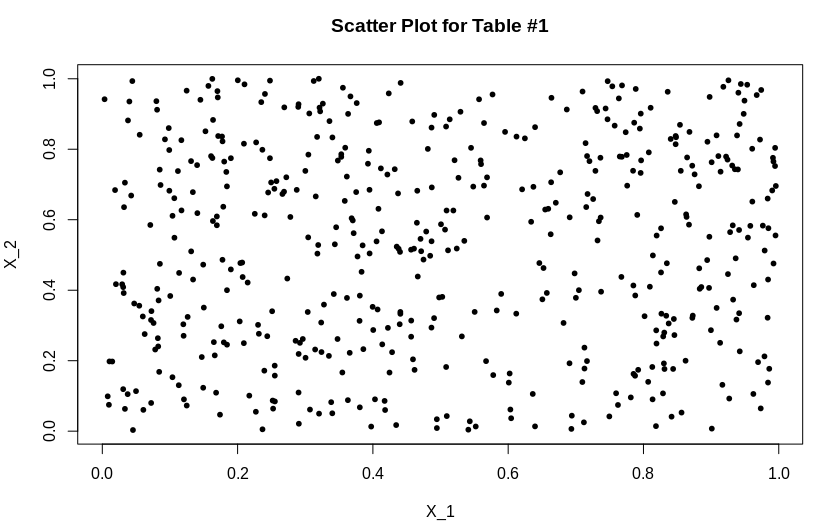
\includegraphics[width=6cm]{X.png}}
			\hfill
			\subfigure[Scatter Plot for table 2]{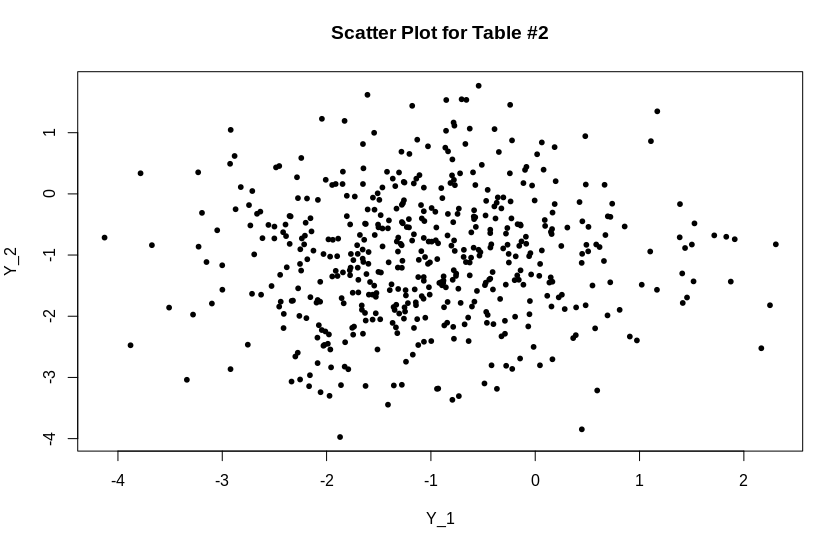
\includegraphics[width=6cm]{Y.png}}
			\hfill
			\centering
			\subfigure[Scatter Plot for table 3]{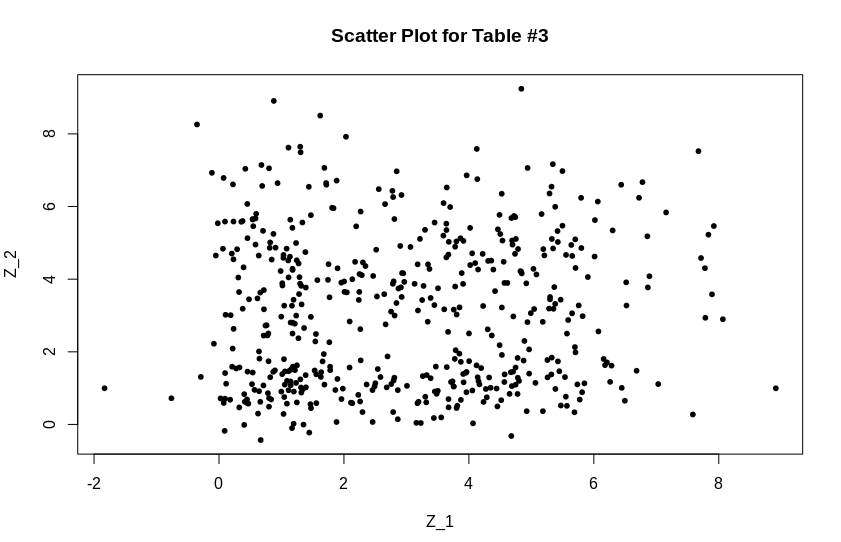
\includegraphics[width=6cm]{Z.png}}
			\hfill
			\caption{Scatter Plots}
		\end{figure}  
		As we can see from Figure 1 above, none of the tables appear to have any type of correlation from a visual inspection.
	\section{Covariance}
		At this level of our analysis, we computed the covariance for each set of data and we obtained the following:
		\begin{itemize}
			\item Table1: cov(x, y) = 0.006
			\item Table2: cov(x, y) = 0.056
			\item Table3: cov(x, y) = 0.218
		\end{itemize}
		The covariance calculated above simply tells us for each set, by how much in average values of two variables differ from their respective means. 
	\section{Pearson's R and $R^2$}
		Since the 3 data sets are relatively large (number of entries $> 30$), we assumed that they are normally distributed according to the Central Limit Theorem (CLT) and we applied Pearson's test to all of them and got the following:
		\begin{itemize} 
			\item Table1: 
				\subitem - R = 0.072
				\subitem - $R^2$ = 0.051
				\subitem - p-value = 0.110
			\item Table2:
				\subitem - R = 0.049 
				\subitem - $R^2$ = 0.002
				\subitem - p-value = 0.273
			\item Table2:
				\subitem - R = 0.052
				\subitem - $R^2$ = 0.003
				\subitem - p-value = 0.243
		\end{itemize} 
		
		\paragraph{Significance:}
			As we can see from the results above, even though all the 3 sets have a non zero Pearson's R, the fact that their p-values are greater that 0.05 indicates that there is no significant correlation between their columns. 
	
	\section{Spearman's Rho}
		Spearman's rho is a non-parametric correlation which is usually used when the data do not meet parametric assumptions. However, we computed the Spearman's correlation coefficient for each of the 3 sets just to confirm  the results found in section 4 and we obtained the following:
		\begin{itemize}
			\item Table1: 
			\subitem - R = 0.070
			\subitem - p-value = 0.117
			\item Table2:
			\subitem - R = 0.062 
			\subitem - p-value = 0.163
			\item Table2:
			\subitem - R = 0.058
			\subitem - p-value = 0.196
		\end{itemize}
		\paragraph{Significance:}
		Just like with Pearson's R the results above show that, even though all the 3 sets have a non zero Spearman's R, the fact that their p-values are greater that 0.05 indicates that there is no significant correlation between their columns.
	
	\section{Bootstrapping}
		Bootstrapping is another method that can be used to deal with data that do not meet parametric assumptions. However, we bootstrapped the 3 data sets first to obtained their standard errors based on bootstrap samples and second to confirm the results found in section 4. We obtained the following:
			\begin{itemize}
				\item Table1: 
				\subitem - SE = 0.042
				\subitem - confidence interval: Normal = (-0.012, 0.154) 
				\subitem - confidence interval: Basic = (-0.013, 0.151)
				\subitem - confidence interval: Percentile = (-0.008, 0.157)
				\subitem - confidence interval: BCa = (-0.011, 0.153)
				\item Table2:
				\subitem - SE = 0.041 
				\subitem - confidence interval: Normal = (-0.032, 0.130)
				\subitem - confidence interval: Basic = (-0.032, 0.126)
				\subitem - confidence interval: Percentile = (-0.028, 0.130)
				\subitem - confidence interval: BCa = (-0.028, 0.130)
				\item Table2:
				\subitem - SE = 0.046
				\subitem - confidence interval: Normal = (-0.039, 0.143)
				\subitem - confidence interval: Basic = (-0.034, 0.146)
				\subitem - confidence interval: Percentile = (-0.042, 0.138)
				\subitem - confidence interval: BCa = (-0.044, 0.136)
			\end{itemize}
		\paragraph{Significance}
		As we can see from the results above, we received 4 confidence intervals for each data set after bootstrapping. However, we can see that all those intervals cross zero. This means that the direction of the correlation in the original set is not necessarily the same as the direction of the correlation in the bootstrap samples. Which confirms that there is no significant correlation between the columns of the 3 original data sets.
	
	\section{conclusion}
		After performing a Pearson's test, Spearman's test and bootstrapping on the 3 data sets that were provided to us for seminar 3, we can conclude that there is no significant correlation between the 2 columns of each of those sets.
	
\end{document}